\chapter{An information-theoretic account of fragment usage}
\label{sec:chapter-infotheory}

The second part of this book addresses the question of why speakers use fragments at all, and more specifically under which circumstances they prefer to utter a (particular) fragment rather than a full sentence. The theoretical literature discussed in Chapter \ref{sec:chapter-theories} is not concerned with this issue. In generative\is{Generative grammar} syntax, usage preferences are often considered to be irrelevant to syntactic theory \citep[see e.g.][]{newmeyer2003}, since historically the goal of this line of research is to develop a model that generates grammatical utterances but not ungrammatical ones.%
%
\footnote{\citet{bergen.goodman2015} provide an account of fragment usage, which is theoretically relatively closely related to my research, but as I discuss below in Section \ref{sec:fragments-game}, their study is based on a very small and artificial data set.}\afterfn%
%
Some theories of fragments make predictions with respect to the licensing conditions of fragments. For instance, according to the in situ deletion\is{In situ deletion account} account \citep{reich2007}, fragments are licensed by a salient implicit or explicit QuD\is{Question under Discussion}. However, licensing is only a necessary but not a sufficient condition for ellipsis to actually occur: Expressions which are given in the QuD\is{Question under Discussion} and not focused \textit{can} be omitted, but they do not need to be omitted, as the felicitousness of sentential answers to \textit{wh}-questions trivially shows. Therefore, in order to explain usage preferences, there needs to be an additional mechanism that determines whether a speaker chooses a full sentence or a fragment in order to get her message across. 

In this chapter I propose an account of such a mechanism, whose predictions are tested with a rating\is{Acceptability rating task} and a production study\is{Production task} in Chapter \ref{sec:chapter-infotheory-experiments}. I pursue the idea that the choice between two or more ways of encoding a message is constrained by information-theoretic\is{Information theory} \citep{shannon1948} processing principles. Throughout the remainder of this book, the term \textit{signal} refers to an individual utterance that can be used to communicate a proposition. The term \textit{message} refers to the proposition that the speaker wants to communicate. I understand the term \textit{message} as including those pragmatic inferences that contribute to truth-conditional meaning, which are called \textit{explicatures} in relevance theory\is{Relevance theory} \citep{sperber.wilson1995}. This concept comprises e.g. the resolution of deixis and anaphors, but not further pragmatic inferences, like implicatures. A message may therefore be conveyed by different signals, but a signal can also convey different messages. The latter point is particularly relevant in case of fragments, whose interpretation depends on how the omissions are resolved.

The central prediction of my account of fragment usage is that, given a set of grammatical utterances that can be used to communicate a message, the utterance that is most well-formed with respect to the information-theoretic\is{Information theory} principle of Uniform Information Density\is{Uniform Information Density} (UID, \citenob{levy.jaeger2007}) is chosen to communicate this message. Information theory\is{Information theory} is a promising framework for modeling omissions in fragments, because it has been shown to account for the distribution of omission and reduction phenomena at different levels of linguistic analysis. Two constraints on linguistic variation follow from information theory\is{Information theory}: First, more frequent messages will receive shorter signals on average. Second, the internal structure of the message will be optimized by distributing information\is{Shannon information} uniformly at the maximal relatively error-free transmission rate. This imposes an upper bound on the densification of the utterance and can provide an explanation for why omission is sometimes dispreferred even when it is licensed. I pursue the idea that a major reason for this distribution of optional reductions is that the Shannon information\is{Shannon information} of an expression indexes its processing effort\is{Processing effort} \citep{hale2001} and that distributing processing effort\is{Processing effort} uniformly makes the most efficient use of the limited cognitive resources\is{Processing effort} that are available to the hearer.

This chapter is organized as follows. Section \ref{sec:infotheory-noisy-channel} provides a brief overview of information theory\is{Information theory} as it was originally introduced by \citet{shannon1948}, before I outline the specific predictions that information-theoretic\is{Information theory} constraints make on the usage and form of fragments  in Section \ref{sec:infotheory-language}.

\section{Information theory}
\label{sec:infotheory-noisy-channel}
\is{Information theory|(}
Information-theoretic\is{Information theory} concepts have been applied to diverse linguistic phenomena, but when \citet{shannon1948} developed the theory in the middle of the twentieth century, it was not intended to explain phenomena of natural language production and comprehension. \citeauthor{shannon1948} was concerned with efficient communication across a noisy channel\is{Noisy channel} from an engineering perspective, for instance, he lists several techniques, such as telegraphy, telephony, radio or television that he assumed his theory would apply to. In this section I sketch the fundamental aspects of the theory that are relevant to its application to (psycho)linguistic questions in Section \ref{sec:infotheory-language}.

From a linguistic perspective, the \textit{information}\is{Shannon information} conveyed by a linguistic expression might be intuitively thought of as related to its meaning: For instance, processing an utterance like \Next modifies the Common Ground \citep{stalnaker2002} by adding the proposition that the sentence encodes, a set of presuppositions and possibly further pragmatic inferences. One might think that utterances are more informative\is{Shannon information} the more information they add to the Common Ground.

\ex. The pub at the corner serves burgers and chicken wings.

The information-theoretic\is{Information theory} definition of \textit{information}\is{Shannon information}, however, is actually simpler. As \citet[379]{shannon1948} himself puts it, ``semantic aspects of communication are irrelevant to the engineering problem'' of getting a message across the channel. Instead, \citeauthor{shannon1948}'s notion of information is solely determined by the probability of a message to appear in context.%
%
\footnote{\citet{bar-hillel.carnap1953} proposed a semantic extension of the theory, but I restrict myself to \citeauthor{shannon1948}'s version because this is in line with the current research in the field.}\afterfn%
%
The less likely a message is, the more informative\is{Shannon information} it is, and vice versa. When applied to the sentence level, this idea is relatively intuitive, because unlikely messages require a larger update of the hearer's assumptions about the state of the world, or of the Common Ground. For instance, a sentence that describes stereotypical situations, like \Last, or even \Next[a], will appear to be less informative\is{Shannon information} than one that describes surprising situations \Next[b]. If a default hearer does not know anything about this pub in particular, she will assume that it is almost certainly true that they serve beer, very likely that they serve regular pub food, but unlikely that they serve Japanese cuisine.

\ex. \a. The put at the corner serves beer.
     \b. The pub at the corner serves tempura and ramen.

In principle, Shannon information\is{Shannon information} could be quantified on a scale between 0 and 1 encoding the probability of a message given a probability distribution over all messages that are possible in the situation. In that case, a lower value on the scale would be equivalent to higher information\is{Shannon information}. A message that is the only option to be uttered in a context has a probability of 1 and an impossible one has a probability of 0. Instead of the absolute likelihood, \citeauthor{shannon1948} proposes to use the negative logarithm of the event probability, which he argues to be more suitable for various reasons, such as mathematical and practical usefulness.%
%
\footnote{In linguistics, given the large set of possible outcomes (e.g. possible sentences), the probability of an individual sentence, word or morpheme often turns out to be very low. In statistical analyses, such variables are often highly skewed and can be transformed into a (more) linear relationship by log-transformation, that e.g. linear mixed effects models \citep{bates.etal2015} presuppose. Furthermore, \citet{smith.levy2013}  observe that the relationship between corpus\is{Corpus} frequency (i.e. probability) and reading time is logarithmic (but cf. \citet{brothers.kuperberg2019}). This empirically supports the log-transformation of bare probabilities.  }\afterfn%
%
\citeauthor{shannon1948} uses the base 2, so that information\is{Shannon information} is measured in bits according to the formula in Equation \ref{eq:surprisal}. Inverting the polarity has two effects: First, information\is{Shannon information} is never negative, because $p(message|context)$ cannot be negative or larger than 1; and second, the amount of information\is{Shannon information} is larger the less likely a message is. In the psycholinguistic literature, this concept of information\is{Shannon information} is often referred to as \textit{surprisal}, and I will also use both terms interchangeably in what follows.%
%
\footnote{The term \textit{Surprisal}\is{Shannon information} was introduced by \citet{hale2001}, who in turn attributes it to \citet{attneave1959} and accounts for the fact that unexpected messages appear as surprising to the hearer and require more processing effort\is{Processing effort} (see Section \ref{sec:infotheory-effort} for details).}\afterfn%

\begin{equation}
I = \log_2 \frac{1}{p(message\mathbin{|}context)} = - \log_2 p(message\mathbin{|}context) \label{eq:surprisal}
\end{equation}

I illustrated the relationship between probability and information\is{Shannon information} on the basis of sentences, but the definition in \ref{eq:surprisal} can be straightforwardly applied to expressions on any level of linguistic representations. \is{Context, linguistic|(}For instance, on the word level, the information\is{Shannon information} of \textit{beer} in \Last[a] can be calculated as shown in Equation \ref{eq:beer}. Similarly, the information\is{Shannon information} of a phoneme within a word or the likelihood with which  of a specific part of speech follows another one can be quantified.\is{Context, linguistic|)}

\begin{equation}
 I(beer) = - \log_2 p(beer\mathbin{|}the\; pub\; at\; the\; corner\; serves)\label{eq:beer}
\end{equation}

The specific predictions that information theory\is{Information theory} makes with respect to the well-formedness of linguistic expressions result from an interaction of this probabilistic notion of information\is{Shannon information} with the assumption that communication occurs through a \textit{noisy channel}\is{Noisy channel}, which is a crucial part of the communication system that \citet{shannon1948} assumes. Figure \ref{fig:shannon-cystem} illustrates this system. In \citeauthor{shannon1948}'s original framework of communication through a technical device, he defines the components of the system roughly as follows: The \textit{information\is{Shannon information} source} produces the message to be sent, whose form is determined by the modality of communication. For instance, it can range from a sequence of letters in telegraphy to functions over time of different complexity, like an acoustic signal in telephony or spatial coordinates and color in the case of television \citep[380--381]{shannon1948}. The \textit{transmitter} encodes the message into a format that allows it to be sent over the channel. The encoded message is termed the \textit{signal}, which can consist of electric impulses in telephony or sequences of dots, dashes and spaces in telegraphy \citep[382]{shannon1948}. The signal is sent to the \textit{receiver} over the \textit{channel}. In \citeauthor{shannon1948}'s examples, the channel can be the wire or cable the signal is sent across. The receiver has to decode the incoming signal, that is, to convert it back into the original format. The message is then interpreted by the \textit{destination}, which is the intended recipient.

\begin{figure}[t]
 \begin{tikzpicture}[align=center, scale = .8]
 %%% Boxes
  \draw (0,0) rectangle (1.8,1.8);
  \draw (2.8,0) rectangle (4.6,1.8);
  \draw (6.45,.55) rectangle (7.15,1.25);
  \draw (9,0) rectangle (10.8,1.8);
  \draw (11.8,0) rectangle (13.6,1.8);
  \draw (5.9,-1.3) rectangle (7.7,-3.1);
%%% Arrows
 \draw [-{Latex[length=1mm,width=1.5mm]},line width=.2mm] (1.9,.9) -- (2.7,0.9);
 \draw [-{Latex[length=1mm,width=1.5mm]},line width=.2mm] (4.7,.9) -- (6.35,0.9);
 \draw [-{Latex[length=1mm,width=1.5mm]},line width=.2mm] (7.25,.9) -- (8.9,0.9);
 \draw [-{Latex[length=1mm,width=1.5mm]},line width=.2mm] (10.9,.9) -- (11.7,0.9);
 \draw [-{Latex[length=1mm,width=1.5mm]},line width=.2mm] (6.8, -1.2) -- (6.8,.45);

%%% Labels
 \node at (.9,2.4){\textsc{Information}\is{Shannon information}\\[-2pt]\textsc{Source}};
 \node at (3.7,2.15){\textsc{Transmitter}};
 \node at (9.9,2.15){\textsc{Receiver}};
 \node at (12.7,2.15){\textsc{Destination}};
 \node at (2.3,-0.35){\textsc{Message}};
 \node at (11.3,-0.35){\textsc{Message}};
 \node at (5.665,.25){\textsc{Signal}};
 \node at (7.9,.0){\textsc{Received}\\[-2pt]\textsc{Signal}};
 \node at (6.8,-3.6){\textsc{Noise}\\[-2pt]\textsc{Source}};
 \end{tikzpicture}
\caption{Shannon's model of communication \citep[381]{shannon1948}. \label{fig:shannon-cystem}}
\end{figure}

On an abstract level, encoding consists in assigning a signal to each possible message, and depending on which signal is assigned to which message, communication can be more or less efficient.  \citeauthor{shannon1948} distinguishes two properties of the channel that constrain the optimal form of signals to be sent through it, which must be considered by an encoding strategy in order to communicate efficiently.

\is{Noisy channel|(}First, the channel can be (and in practice most of the time is) noisy: Random noise can corrupt the signal during the transmission process, so that the signal passed to the recipient can differ from that sent by the source. For instance, if the signal consists in a sequence of letters A, B, and C, noise could transform a sent signal ABCA into ABBB. \citet[410]{shannon1948} observes that noise potentially constitutes a problem for communication, but that ``by sending the information\is{Shannon information} in a redundant form the probability of errors can be reduced.'' An example of redundant encoding is to send each letter four times. For the above signal, this yields AAAABBBBCCCCAAAA. If now only one of the four repetitions of each letter was corrupted by noise on average, the intended letter could still be recovered by assuming that the most frequent letter in each substring is the one intended by the sender. Of course, this encoding strategy makes communication less efficient: If the signal length is increased by the factor $n$, sending it will take $n$ times longer than sending the short signal. Therefore, efficient coding will involve a trade-off between the transmission of as much information\is{Shannon information} as possible in a given interval of time and minimizing the probability of errors by including additional redundancy. Second, the channel has a limited \textit{channel capacity}\is{Channel capacity}, which is measured in bits transmitted per unit of time. \citet[401--413]{shannon1948} shows that, given an appropriate coding system, information\is{Shannon information} can be transmitted with a very low error rate unless the transmission rate does not exceed channel capacity\is{Channel capacity}. However, when channel capacity\is{Channel capacity} is exceeded, the likelihood of errors increases faster than the gain in intended transmission rate. Hence, attempts of increasing the transmission rate above channel capacity\is{Channel capacity} will never yield an advantage, but further reduce the actual transmission rate.

Taken together, in order to communicate efficiently across a noisy channel\is{Noisy channel}, the best choice is to communicate at a rate close to but not exceeding channel capacity\is{Channel capacity}: Not making use of the available bandwidth would be inefficient and more time-consuming, while exceeding channel capacity\is{Channel capacity} harms the purpose of communication due to the increased likelihood of errors and, as \citeauthor{shannon1948} shows, will not yield an effectively higher transmission rate. In simplified terms, this requires interlocutors to allow for a certain degree of redundancy in their signal whenever channel capacity\is{Channel capacity} would be exceeded otherwise. As long as this is not the case, they should densify their utterance as much as possible in order to maximize efficiency.\is{Noisy channel|)}\is{Information theory|)}

On an abstract level, the idea that underlies information-theoretic\is{Information theory} research on language is that these general constraints on communication can explain optional variation in language. Grammar often provides a variety of signals that can be used to communicate a message, but does not explain why speakers choose a particular one in a specific situation. Specifically in the case of ellipsis, grammar determines whether an omission is licensed, but not all omissions that are licensed necessarily occur. From an information-theoretic\is{Information theory} perspective, a perfectly grammatical utterance might be dispreferred as compared to another one, for instance, because it is too redundant or because it exceeds channel capacity\is{Channel capacity}. This idea is worked out in detail in what follows.

\section{Information-theoretic constraints on language}
\label{sec:infotheory-language}

The model of communication in Figure \ref{fig:shannon-cystem} that \citet{shannon1948} assumes can easily be translated to any communicative situation between two interlocutors. Just like in the model, the speaker first has to  encode her message, which can be thought of as a proposition, into an acoustic or written signal. This signal is sent across an acoustic or visual channel to the hearer, who has to decode, i.e. parse\is{Parser, human} and interpret it. During the transmission process, the signal can be corrupted by noise\is{Noisy channel|(}. As I discuss in greater detail below, noise can be thought of as acoustic noise in the environment or as any other factor that results in a difference between the message sent by the speaker and the message received by the hearer.\is{Noisy channel|)} In principle, utterances can be optimized with respect to the properties of the communication system on any level of linguistic analysis, be it phonemes, morphemes, words, more abstract syntactic constructions or complete sentences.

The account of fragment usage that I propose assumes that interlocutors optimize their utterances with respect to the goal of communicating efficiently through a noisy channel\is{Noisy channel}, as has been shown by previous research on information-theoretic\is{Information theory} constraints on language. Applied to natural language, the encoding process consists in assigning a linguistic signal, i.e. an utterance, to the intended message, that is, the proposition to be communicated. In the case of the choice between fragment and sentential utterances this optimization can involve the optional omission of words in the utterance, which might result in a preference for the fragment.

\is{Source coding|(}\is{Channel coding|(}For the purpose of efficient communication, the encoding process must consider the properties of the components of the communication system. Previous research has identified two components of the model with respect to whose properties the signal is optimized: the source\is{Source coding} and the channel\is{Channel coding}. Most of the recent work on information theory\is{Information theory} in psycholinguistics, in particular studies on the UID\is{Uniform Information Density} hypothesis \citep{levy.jaeger2007}, focus on adaptation to properties of the channel. Even before that, \citet{zipf1935}\is{Zipf's Law} observed a relationship between the frequency and length of linguistic expressions which suggests that statistical properties of the source\is{Source coding} also constrain encoding preferences. As \citet{pate.goldwater2015} show, the optimization of the signal to properties of the source, which they term \textit{channel coding}\is{Channel coding} and \textit{source coding}\is{Source coding} make partially differing predictions. In order to specify testable predictions of information theory\is{Information theory} on the form and usage of fragments, effects of source and channel coding have to be teased apart. 

In what follows I discuss the predictions of source and channel coding on the form of utterances. It will become evident that both of these strategies predict that more frequent messages are more likely to be reduced, but only channel coding predicts the insertion of additional redundancy, the adaptation to the communicative situation and hence to the hearer's expectations.%
\footnote{My experiments do not investigate the adaptation to the communicative situation. For evidence with respect to this see e.g. \citet{pate.goldwater2015}.}\afterfn%
%
Furthermore, in the case of fragments, only channel coding\is{Channel coding} makes explicit predictions about \textit{which} words are omitted and which ones are realized. These are the predictions which I test in the two experiments in Chapter \ref{sec:chapter-infotheory-experiments}.\is{Source coding|)}\is{Channel coding|)}

\subsection{Source coding}
\label{sec:infotheory-zipf}
\is{Source coding|(}

In \citepos{shannon1948} terminology, the source is the part of the communication system that generates messages, which then have to be encoded in order to be sent over the channel. Source coding\is{Source coding} focuses on the probability distribution over possible messages. In applications of information theory\is{Information theory} to linguistic phenomena the possible messages will differ in their likelihood most of the time. For instance, in a pub scenario, it is relatively likely that the customer will order drinks and food (in particular specific types thereof), but less likely that he wants to tell the waiter about an interesting linguistic paper that he recently read.\is{Context, extralinguistic} As I discussed in Section \ref{sec:infotheory-noisy-channel}, encoding consists in assigning a signal to each message, and most of the time the expressions that are available in the set of possible signals differ in length. In this situation, an efficient source coding strategy reserves the shorter signals for likely messages and assigns longer signals to unlikely ones \citep[402]{shannon1948}. This reduces the average length of an actually produced signal on average, because it ensures that shorter signals are sent more often.

\is{Zipf's Law|(}
Source coding\is{Source coding} effects have been reported specifically on the word level, since \citet{zipf1935}\is{Zipf's Law} observed that more frequent words tend to be shorter on average in English\il{English}, Latin and Chinese\il{Chinese}.%
%
\footnote{\citeauthor{zipf1935} himself refers to \citet{kaeding1897} and \citet{eldridge1911} for previous tentative evidence in favor of this hypothesis. \citet[23--25]{zipf1935} however argues that for methodological reasons neither of these studies ultimately confirms the hypothesis.}\afterfn%
%
This motivates his Law of Abbreviation, which states that ``as the relative frequency of a word increases, it tends to diminish in magnitude.'' He argues that this principle results from a tendency toward ``saving of time and effort'' \citep[38]{zipf1935}. The number of possible short words in a language is naturally restricted by the limited inventory of phonemes and the syllabic structure of that language. Assigning shorter signals to more frequent messages reduces the average length of a random word as compared to a hypothetical language where there is no correlation between frequency and length. Consequently, the length-frequency correlation allows for the transmission of more words in less time, or, in the case of written speech, space.%
%
\footnote{\citet[30-36]{zipf1935} relates diachronic changes, like the shortening of \textit{gasoline} to \textit{gas} and the substitution of \textit{automobile} by \textit{car}, to an adaption to the increased frequency of these words.}\afterfn%
%
More recently, \citepos{zipf1935} observation has been replicated for a larger sample of languages by \citet{piantadosi.etal2011} and for semantically similar words that differ in length (e.g. \textit{math} vs. \textit{mathematics}) by \citet{mahowald.etal2013}.%
%
\footnote{\citet{mahowald.etal2018} furthermore show that across a variety of languages, even when word length is controlled, more frequent words have more phonotactically probable forms than less frequent ones.}\afterfn%
%
\is{Zipf's Law|)}

The idea that shorter signals are assigned to more frequent, i.e. likely, messages can be extended to the sentence level. Source coding\is{Source coding} then predicts that more frequent messages are preferably encoded as a fragment. Unlikely messages will rather be encoded as a full sentence if all of the shorter fragments have already been allocated to more likely messages. \is{Context, extralinguistic|(}For instance, consider an extremely simplified taxi scenario, which models the communicative situation after a pedestrian (the speaker) hailed a taxi. In the scenario, there are only two messages that differ in their probability \Next%
%
\footnote{For expository purposes, I do not provide semantic representations in this case, but simply a paraphrase of the speaker's communicative intention.}\afterfn%
% 
and three signals that differ in length \NNext, including a fragment \NNext[c]. Since the fragment can be derived from both \NNext[a] and \NNext[b], it can encode both messages in \Next. A speaker who performs source coding\is{Source coding} will assign the fragment to the more probable message \Next[a], so that the only way of encoding the less informative\is{Shannon information} message in \Next[b] is the less informative\is{Shannon information} full sentence in \Next[b].\is{Context, extralinguistic|)}

\ex. Messages
\a. The pedestrian wants a ride to the university.\hfill $p = a;\;a > 0.5$
     \b. The pedestrian wants to know how to get to the university. \hfill$p = 1-a$

\ex. Signals
\a. Take me to the university, please! \hfill $length = 6$
     \b. Explain me the way to the university, please! \hfill $length = 8$
     \c. To the university, please!\hfill $length = 4$

Source coding\is{Source coding} consequently predicts that more likely messages are more often encoded as fragments, but this does not necessarily imply that less likely messages are preferably encoded as full sentences: In a hypothetical situation with very few possible messages, as long as there is a sufficient number of fragments to encode all messages, none of the messages will be encoded as a sentence. Source coding\is{Source coding} thus predicts no upper bound on densification: If unpredictable messages receive longer signals, this is only a by-product of the assignment of short signals to predictable messages, as the taxi example illustrated.\is{Source coding|)}

Source coding\is{Source coding} on the sentence level also makes no predictions on the internal form of the signal. It can explain why fragments are more often used to communicate predictable messages, but it cannot explain why specific words are omitted in these fragments. As will become evident throughout the next section, this is predicted only by channel coding\is{Channel coding} accounts like Uniform Information Density\is{Uniform Information Density}.

\subsection{Channel coding}
\label{sec:infotheory-uid}
Focusing on the source alone disregards the idea that the signal is transmitted over a noisy channel\is{Noisy channel} with limited capacity\is{Channel capacity} in \citeauthor{shannon1948}'s model: Speakers should not only optimize their utterance with respect to properties of the source\is{Source coding}, but also with respect to those of the channel. In particular, they should avoid exceeding or repeatedly underutilizing the available capacity\is{Channel capacity}. This requires them to keep track of the distribution of information\is{Shannon information} across the signal. Channel coding\is{Channel coding} predicts a preference for those signals that ensure a transmission rate below but close to channel capacity\is{Channel capacity}. This is the main difference between the prediction between source and channel coding, because source coding\is{Source coding} imposes no such upper bound on the densification of the signal.

\subsubsection{Uniform Information Density}
\is{Channel coding|(}
In the literature, channel coding\is{Channel coding} has been discussed under different labels. In what follows, I sketch the general idea, its psychological reality and methods used to investigate its empirically testable predictions.

The idea that speakers adapt their utterance to the channel has been applied to linguistic phenomena for the first time by \citet{fenk.fenk1980}, \citet{fenk-oczlon1989} and \citet{fenk-oczlon1990} even before the more recent rise of information-theoretic\is{Information theory} accounts of language processing in psycholinguistics. \citet{fenk.fenk1980} proposed a principle of \textit{Constant Flow of Information}\is{Shannon information}, which states that the amount of information sent by unit of time\is{Information density} varies only weakly around a constant mean \citep[38]{fenk-oczlon1990}. \citet[403]{fenk.fenk1980} argue that increasing the rate of transmission too far above this mean would exceed the processing capacity\is{Processing effort} of the hearer, whereas falling below the mean would be inefficient. This approach models channel capacity\is{Channel capacity} as an upper bound on the cognitive resources\is{Processing effort} of the hearer, an idea that I also adopt in this book (see Section \ref{sec:infotheory-effort} for details).

\is{Uniform Information Density|(}
More recently, the idea that speakers tend toward distributing information\is{Shannon information} uniformly across the speech signal has been reformulated for different levels of linguistic analysis. For instance, the \textit{Smooth Signal Redundancy} hypothesis by \citet{aylett.turk2004} predicts that speech is smoothed on the phonetic level by modulating the length of syllables. On the level of complete sentences, \citet{genzel.charniak2002, genzel.charniak2003} propose an \textit{Entropy\is{Entropy} Rate Constancy} principle, which states that the average entropy\is{Entropy} of sentences throughout a text is constant. Whereas these principles are related to specific levels of analysis, \citet[24]{levy.jaeger2007} explicitly claim that their \textit{Uniform Information Density}\is{Uniform Information Density} (UID) hypothesis holds on any level of analysis. Work relying on the notion of UID has mostly focused on morphosyntactic variation, such as contractions \citep{frank.jaeger2008} and omissions of function words \citep{levy.jaeger2007, jaeger2010} as well as grammatical markers \citep{kurumada.jaeger2015, norcliffe.jaeger2016}, which will turn out to be particularly relevant to the investigation of omissions in fragments. For this reason, I will use the notion of UID in order to refer to the principle of distributing Shannon information\is{Shannon information} as uniformly as possible across the utterance.

On an abstract level, UID\is{Uniform Information Density} predicts that if there are several signals that can encode a message, everything else being equal, the speaker will choose the signal which comes closest to the ideal distribution of information\is{Shannon information}\is{Information density}, which approximates channel capacity\is{Channel capacity} without exceeding it. At least in the original version of the theory, the set of possible signals is restricted to grammatical expressions, since \citet[25]{jaeger2010} argues that optional variation occurs only within ``the bounds defined by grammar.'' This assumption is crucial to the empirical investigation of fragments, because it implies that UID\is{Uniform Information Density} favors the most well-formed \textit{grammatical} signal and does not take into account utterances that might distribute information\is{Shannon information} even more uniformly but that cannot be derived by grammar.

Following \citet[849]{levy.jaeger2007}, the \textit{information\is{Shannon information} density\is{Information density}} of an utterance is defined as ``the amount of information\is{Shannon information} per unit comprising the utterance'', that is, the sum of the information\is{Shannon information} carried by each individual word within the utterance. This total information\is{Shannon information} density\is{Information density} mass is to be distributed as uniformly as possible across the words comprising the utterance. Distributing information\is{Shannon information} uniformly implies that speakers ``avoid peaks and troughs in information\is{Shannon information} density\is{Information density}'' \citep[849]{levy.jaeger2007}, which result from transmitting too little or too much information\is{Shannon information} per unit of time. In that sense, troughs are local information\is{Shannon information} minima that result in an inefficient use of channel capacity\is{Channel capacity}, whereas peaks are information maxima that exceed channel capacity\is{Channel capacity} and therefore hamper communication. %
\is{Channel coding|)}
\is{Uniform Information Density|)}

\subsubsection{UID effects on omissions}
In order to illustrate how omissions in fragments may contribute to the optimization of utterances with respect to UID\is{Uniform Information Density}, consider again the taxi example that I discussed above. In this situation, a pedestrian hails a taxi, because he needs a ride to the university. In this simplified example, he can in principle choose between a full sentence \Next[a] and a fragment \Next[b] to communicate this message.%
%
\footnote{Of course, this is highly simplified, because he could make use of a wide variety of different syntactic constructions and lexicalizations of fragments and sentences.}\afterfn%
% 

\ex. \label{ex:uid-taxi}
\a. Take me to the university, please.
     \b. To the university, please.

In the taxi scenario it will be in general very likely\is{Context, extralinguistic} that the passenger wants to go somewhere, so the material that is omitted in the fragment (\textit{take me}) is very predictable. In contrast, it is unlikely that the driver knows the passenger's destination, this destination is unpredictable and relatively informative. Figure \ref{fig:fragments-uid-predictable}, which shows the distribution of information\is{Shannon information} over time,%
%
\footnote{The variable on the abscissa in principle is time, because channel capacity\is{Channel capacity} and transmission rates are defined as an amount of information\is{Shannon information} transmitted per unit of time, e.g. in bits per second. In practice, however, specifically corpus\is{Corpus}-based work \citep[see e.g.][]{levy.jaeger2007, frank.jaeger2008, jaeger2010} simplifies this to the amount of information\is{Shannon information} transmitted per word, because duration measures for words or appropriate transcriptions into phonemes are not available in the corpora\is{Corpus} or would complicate the statistical analysis.}\afterfn%
%
illustrates this idea with hypothetical information density\is{Information density} (ID) profiles for the fragment and the corresponding full sentence. 

\begin{figure}[t]
\begin{minipage}{\textwidth}
\begin{tikzpicture}
 \node at (0,0) {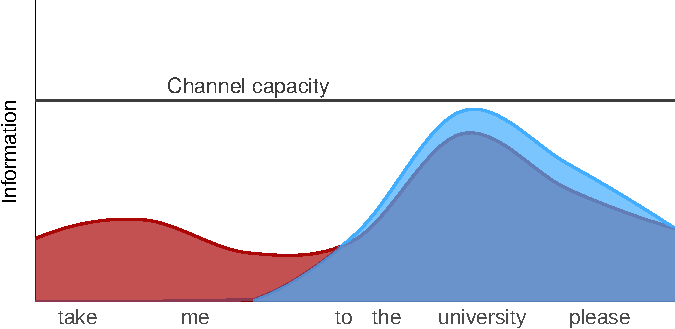
\includegraphics[scale=1]{figures/uid-example-fragment}};
 \node at (0.5,-2) {\large \sffamily Take~~~~~~~~~~ me ~~~~~~~~~~~~~~~~~~~~to~~~~~ the ~~~university ~~~~~~~~ please};
\end{tikzpicture}
\end{minipage}
 \caption{Hypothetical ID profile for the predictable sentence \textit{take me to the university} and the meaning-equivalent fragment \textit{to the university} in the taxi scenario. The blue area illustrates the distribution of information in the fragment and the red area that in the full sentence.\label{fig:fragments-uid-predictable}}
\end{figure}

\is{Context, extralinguistic|(}If the pedestrian wants the driver to tell him the way to the university instead, he has to choose between the fragment in \Last[b] and the sentence in \Next. In that case, \textit{tell me the way} is probably less predictable than \textit{take me}, as Figure \ref{fig:fragments-uid-unpredictable} suggests. Of course, whether a word is predictable depends on properties of the utterance context. For instance, when an utterance like \Next is not produced by a passenger approaching the taxi, but by the driver of another car with a foreign license plate, it might be more likely that he would ask the local taxi driver for the way than that he wants to go somewhere. Similarly, when the passenger is brought to the university by the same driver on every Wednesday, or he wears a Denver Nuggets hat and shirt an hour before the match starts, the destination might be more likely and the utterance possibly even further reduced.\is{Context, extralinguistic|)} %

\ex. Tell me the way to the university, please.

\begin{figure}[t]
\begin{minipage}{\textwidth}
\begin{tikzpicture}
 \node at (0,0) {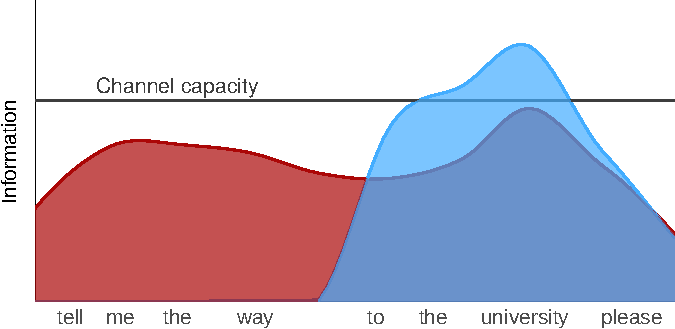
\includegraphics[scale=1]{figures/uid-example-sentence}};
 \node at (0.3,-2) {\large \sffamily Tell~~~~~ me ~~~~~~~the~~~~~~~~~way ~~~~~~~~~~ to ~~ the~~ university~~~ please};
\end{tikzpicture}
\end{minipage}
\caption{Hypothetical ID profile for the unpredictable sentence \textit{tell me the way to the university} and the meaning-equivalent fragment \textit{to the university} in the taxi scenario. The blue area illustrates the distribution of information in the fragment and the red area that in the full sentence.\label{fig:fragments-uid-unpredictable}}
\end{figure}
%
Figure \ref{fig:fragments-uid-predictable} shows how the local information\is{Shannon information} minimum, or \textit{trough}, in the ID profile\is{Information density} that is caused by the redundant \textit{take me} is smoothed by omitting this expression. From a UID\is{Uniform Information Density} perspective, omitting such predictable words optimizes the signal. If these omissions target words that are obligatory in full sentences, this results in the preference of the fragment over the full sentence. In contrast, given the density\is{Information density} profiles in \ref{fig:fragments-uid-unpredictable}, \textit{tell me the way} does not yield a trough in the profile, hence there is no pressure to omit these words. Furthermore, its omission would result in a \textit{peak} in the density\is{Information density} profile that exceeds channel capacity\is{Channel capacity}.%
%
\footnote{Note that Figure \ref{fig:fragments-uid-unpredictable} is not fully accurate, because I assigned the identical fragment \textit{to the university} different density\is{Information density} profiles in the left and right panel for the purpose of illustration. See below in this section for a discussion of this issue.}\afterfn%
%
Therefore, from the UID\is{Uniform Information Density} perspective, it is not beneficial to omit these words. Actually, even if \textit{tell me} was redundant, its insertion is preferred as long as it contributes to reducing the peak on \textit{to the university}. 

The tendencies to (i) to omit predictable expressions and (ii) to realize expressions that reduce peaks on upcoming material are the central predictions of UID\is{Uniform Information Density} on the well-formedness of linguistic expressions. Both of them are empirically supported by previous research, as \citet{frank.jaeger2008} show for contraction in English\il{English}, \citet{kurumada.jaeger2015} for Japanese case markers, \citet{levy.jaeger2007} for relative pronouns in English\il{English}, \citet{jaeger2010} for complementizers, \citet{norcliffe.jaeger2016} for relative pronouns in Yucatec Maya, \citet{asr.demberg2015} for discourse markers and \citet{lemke.etal2017} for articles\is{Article omission}. With the exception of \citet{kravtchenko2014}, who investigates the omission of subjects in Russian\il{Russian}\is{Subject drop}, these studies investigate semantically relatively vacuous function words. It is therefore reasonable to assume that UID\is{Uniform Information Density} constrains omissions in fragments too, but this does not necessarily follow from previous research. The finding by \citet{tily.piantadosi2009} that more predictable nouns are more likely to be pronominalized, i.e. reduced, points in a similar direction, if ellipsis as a more radical form of reduction of given material. Furthermore, the relationship between predictability and reduction has also been evidenced by studies which find that predictable expressions are more likely to be reduced in terms of duration and/or articulatory effort both on the word level and on that of individual syllables \citep[see e.g.][]{bell.etal2003, aylett.turk2004,  bell.etal2009, tily.etal2009, demberg.etal2012, kuperman.bresnan2012, seyfarth2014, pate.goldwater2015, brandt.etal2017, brandt.etal2018,  malisz.etal2018}.

Even though the concept is labeled \textit{Uniform} Information Density, at least in the version adopted in current psycholinguistics, the property of uniformity is an artifact of the assumptions made and not a goal of the encoding strategy in its own right. Uniformity only follows from the approximation of the transmission rate to the channel capacity\is{Channel capacity}, but a uniform distribution far below channel capacity\is{Channel capacity} will still be dispreferred compared to less uniform signals that make a more efficient use of channel capacity\is{Channel capacity}. This leads to an important distinction between the effect of peaks and troughs with respect to the choice between alternative ways of encoding a message. Troughs are inefficient and therefore always to be avoided, if possible. In contrast, peaks only dispreferred if they exceed channel capacity\is{Channel capacity}. In what follows, I will imply this interpretation of uniformity when stating that a signal is more or less compliant to UID\is{Uniform Information Density}, unless stated otherwise.

As for now, there have been no attempts to quantify channel capacity\is{Channel capacity}. This would not be a promising endeavor, because, as \citet{shannon1948} showed, channel capacity\is{Channel capacity} is not a constant, but varies as a function of the noise rate\is{Noisy channel} in the channel. This indeterminacy of channel capacity\is{Channel capacity} is expected if UID\is{Uniform Information Density} is interpreted as a psycholinguistic constraint on communication. UID\is{Uniform Information Density} implies that speakers are engaged in audience design\is{Audience design} and adapt their utterances to expected properties (e.g. preferences and cognitive abilities) of the hearer, so this will necessarily involve inferences under uncertainty about channel capacity\is{Channel capacity}. Furthermore, from a methodological perspective, the absolute information\is{Shannon information} estimate depends on the corpus\is{Corpus} used for this purpose. Since information\is{Shannon information} is based on probabilities, a larger lexicon will result in lower average probabilities of individual items. What matters for empirical research on UID\is{Uniform Information Density} is that, even if channel capacity\is{Channel capacity} is unknown, on average, more informative\is{Shannon information} words are more likely to yield a peak and more uninformative words are more likely to cause a trough in the ID profile\is{Information density}.

Taken together, UID\is{Uniform Information Density} predicts that, given a set of possible signals, i.e. sentential and nonsentential utterances that can be used to encode a message and that comply with grammar,%
%
\footnote{Most of the time, this set of possible signals will be too large to empirically evaluate the alternatives. Even if no fragments were considered at all, a theoretically infinite number of sentences can be used to convey a single message. Therefore, when it comes to evaluating the alternative set empirically, I will assume that there is one sentence equivalent to each message from which a set of fragment alternatives is derived by ellipsis. This concerns in particular the evaluation of the production study\is{Production task} in Section \ref{sec:scripts-production}.}\afterfn%
% 
the preferred utterance is that which distributes information\is{Shannon information} most uniformly across the utterance. This leads to the two specific predictions in \Next[a,b], which in turn imply \Next[c]: If omissions occur more often in predictive contexts, because average words are more likely, the signal will on average be shorter in such situations.

\ex. \textit{Predictions of UID\is{Uniform Information Density} on fragments} \label{ex:uid-fragments-predictions}
\a. \textit{Avoid troughs}: The more likely a word is in context, the more likely it is to be omitted (within the limits of grammar).\label{ex:uid-fragments-predictions-troughs}
 \b. \textit{Avoid peaks}: Uninformative words can be inserted before very informative words in order to lower the surprisal\is{Shannon information} of the latter (within the limits of grammar).\label{ex:uid-fragments-predictions-peaks}
 \c. \textit{Densification}: Shorter signals, like fragments, are preferred in predictive contexts.\label{ex:uid-fragments-predictions-densification}

\subsubsection{UID effects on word order}
\is{Word order|(}
The distribution of information\is{Shannon information} across the signal can also be optimized by reordering the expressions that it comprises. Effects of word order\is{Word order} on UID\is{Uniform Information Density} are not as central to my research question as omissions, because they are not unique to fragments, but my experiment \ref{exp:scripts-production} will also show that there is evidence for UID\is{Uniform Information Density} effects on word order\is{Word order}. \is{Context, linguistic|(}Word order\is{Word order} effects are predicted by UID\is{Uniform Information Density} because a word's information depends on the context in which it occurs and variation of word order changes this context. In general, the larger the context of a word is, the more predictable this word tends to become, because preceding material narrows the range of possible continuations of the utterance. This has also been shown by \citet{levy2008} for verb-final contexts in German\il{German} based on reading time data by \citet{konieczny.doring2003}. The more arguments of the final verb the hearer parses\is{Parser, human}, the smaller does the set of potential completions of the sentence become. This surprisal\is{Shannon information} reduction is reflected in reduced reading times for words that occur later in the clause. \citet{fenk-oczlon1983} argues that this also accounts for the general tendency for given or topicalized expressions to precede new or focused ones \citep{chafe1976}: Given expressions are on average more predictable than new ones, and therefore this ordering reduces the information of the new ones and yields a more uniform ID profile\is{Information density}.\is{Context, linguistic|)}%
%
\footnote{Most of the time, topicality and high predictability will probably cooccur. However, these concepts operate on different levels of analysis. Topicality determines what an utterance is about \citep{reinhart1981, krifka2007} but predictability determines only the likelihood of a word to be mentioned at a particular point within the utterance. Expressions can be predictable, but not topical, if they have are likely in context and they are focused. For instance, in \Next, taken from \citet{kuperberg.etal2020}, the target noun \textit{swimmers} has a high cloze probability as compared to \textit{trainees} or \textit{drawer} -- all of these three words appear in the comment and the topic of the sentence are the lifeguards.

\ex. The lifeguards received a report of sharks right near the beach. Their immediate concern was to prevent any incidents in the sea. Hence, they cautioned the (swimmers/trainees/drawer).

}\afterfn%
% 
More recently, \citet{sikos.etal2017} report an effect of UID\is{Uniform Information Density} on the choice between pre- and postnominal modification of German\il{German} nouns, and \citet{speyer.lemke2017} observe an effect of the aggregated surprisal\is{Shannon information} of relative clauses on their extraposition in historic stages of German\il{German}.

Even though UID\is{Uniform Information Density} predicts effects on word order\is{Word order}, fragments often do not allow for word order\is{Word order} variation. For instance, in a German\il{German} DP\is{Determiner phrase} or PP\is{Preposition phrase}, word order\is{Word order} is relatively fixed and determined by grammar, and UID\is{Uniform Information Density} only determines the choice between grammatical expressions. I return to this issue in the discussion of experiment \ref{exp:scripts-production}, because the data set that I collected in this study is suitable for the investigation of UID\is{Uniform Information Density} effects on optional word order\is{Word order} variation, too.%
%
\footnote{Exceptions to the fixed word order within DPs and PPs are e.g. DPs\is{Determiner phrase} that contain multiple adjectives \Next and a few prepositions that can also appear postnominally \NNext. I leave such variation aside, because in the first case there are semantic and phonological constraints that strongly bias the ordering of adjectives \citep{martin1969, dixon1977, cinque1994, wulff2003}, and postposition \NNext is restricted to single lexical items \citep{dimeola2003}.

\ex. \ag. das neue schnelle Fahrrad\\
	  the new fast bike\\
     \bg. das schnelle neue Fahrrad\\
	  the fast new bike\\
	  \trans{the fast new bike}

\ex. \ag. wegen des Regens\\
	  because the.\textsc{gen} rain.\textsc{gen}\\
      \bg. des Regens wegen\\
	  the.\textsc{gen} rain.\textsc{gen} because\\
	  \trans{because of the rain}

}\afterfn%
%
\is{Word order|)}

\subsubsection{Summary: Predictions of UID on the form of fragments}
UID\is{Uniform Information Density} makes empirically testable predictions with respect to the preferred way of encoding of a message. Speakers use omissions of optional words in order to modulate the information density profile\is{Information density} in two ways: On the one hand, omitting uninformative words can smooth the profile by avoiding troughs. On the other hand, the insertion of redundant words before otherwise unpredictable ones reduces peaks in the profile. Such effects, which will be observed on the word level, are more specific than the general preference to assign shorter utterances to more predictable messages that follows from source coding\is{Source coding}. This relationship between the probability of a message and the length of the signal that source coding\is{Source coding} predicts also results from UID\is{Uniform Information Density}. For predictable messages, the individual words will also be on average more likely, so that there will be a higher ratio of omissions, which in turn results in a shorter signal. While UID\is{Uniform Information Density} and source coding\is{Source coding} share the prediction that shorter signals are assigned to more likely messages, only UID\is{Uniform Information Density} predicts \textit{which} words are omitted in fragments.

\subsection{UID as efficient distribution of processing effort} 
\label{sec:infotheory-effort}
The studies cited above support the basic prediction of UID\is{Uniform Information Density}, that is, the tendency of distributing information\is{Shannon information} uniformly across the utterance. However, in the literature two different ways of mapping the abstract concepts in \citeauthor{shannon1948}'s model of communication to natural language have been suggested. These interpretations differ particularly with respect to the channel. On the one hand, specifically in phonetic research, the channel is interpreted rather literally as the space through which the signal is sent \citep[see e.g.][]{aylett.turk2004}. On the other hand, from a psycholinguistic perspective, the channel has been related to the processing resources\is{Processing effort} available to the hearer, and channel capacity\is{Channel capacity} interpreted as an upper bound to these resources \citep[see e.g.][]{fenk.fenk1980}. Before returning to UID\is{Uniform Information Density} effects on omissions, I briefly review these approaches and argue why I adopt the second possibility and interpret Shannon information\is{Shannon information} as a measure of processing effort, as has been suggested e.g. by \citet{hale2001} and \citet{levy2008}. 

\is{Noisy channel|(}The interpretation of the channel which is more closely related to the communicative situation modeled by \citet{shannon1948} conceptualizes the channel as the medium between speaker and hearer. From this perspective, the message can be corrupted by noise\is{Noisy channel} during transmission and UID\is{Uniform Information Density} ensures ``robust information\is{Shannon information} transfer in a potentially noisy environment while conserving effort'', as \citet[32]{aylett.turk2004} put it. Noise can be acoustic, but it can also consist in other modifications of the signal, like hearers being distracted by other tasks \citep{hauser.etal2019}. As \citet{shannon1948} showed, an increased likelihood of noise reduces channel capacity\is{Channel capacity}, because the potential corruption of the message has to be counterbalanced by inserting additional redundancy. In particular on the phonetic level and in case of high noise ratios this is a reasonable assumption, because the prediction of information\is{Shannon information} theory\is{Information theory} that speakers adapt their utterances in the presence of acoustic noise is a well-established finding, known as the \textit{Lombard effect}  \citep{lombard1911}. Experimental research has shown that this adaptation concerns a variety of parameters, including an increase in F0, speech level and vowel duration \citep{summers.etal1988,junqua1994, junqua1996}. This is in line with information\is{Shannon information}-theoretic studies that find effects of predictability on the articulation and duration of words and phonemes \citep{bell.etal2003, aylett.turk2004, bell.etal2009, brandt.etal2017, brandt.etal2018, malisz.etal2018}.\is{Noisy channel|)}

However, it is unclear whether the assumption that UID\is{Uniform Information Density} effects are related to the presence of environmental noise holds to the same extent for higher levels of linguistic analysis, such as words or complete sentences. In regular face-to-face communication, in the absence of a significant source of acoustic noise, and specifically if the word level is concerned, it seems relatively unlikely that complete are misheard. Words that are similar to each other, like \textit{Harry} and \textit{Mary} might be misunderstood if a part of the word is corrupted by noise, but it is less likely that \textit{Harry} is misunderstood as \textit{Susan} for this reason.

\is{Processing effort|(}The link between predictability and processing effort\is{Processing effort} allows for an interpretation of UID\is{Uniform Information Density} as a strategy to communicate efficiently even in the absence of (perceptual) noise. \citet[850]{levy.jaeger2007} note that ``independently of whether linguistic communication is viewed as a noisy channel\is{Noisy channel}, UID\is{Uniform Information Density} can be seen as minimizing comprehension difficulty.'' This is based on the insight that the effort\is{Processing effort} required to process an expression is proportional to its predictability in context \citep{hale2001, hale2016, levy2005, levy2008}. In psycholinguistics it is a well-established finding that, everything else being equal, more predictable words are read faster \citep[see e.g.][]{ehrlich.rayner1981, mcdonald.shillcock2003, demberg.keller2008, smith.levy2013}. \citet[850]{levy.jaeger2007} relate UID\is{Uniform Information Density} and processing effort\is{Processing effort} by suggesting that a uniform distribution of information\is{Shannon information} minimizes the total processing effort\is{Processing effort} of an utterance, which they define as the sum of the processing effort\is{Processing effort} of all the words within this utterance.%
%
\footnote{There is some disagreement in the literature on the scale on which processing effort\is{Processing effort} and word probability are related. \citet{levy.jaeger2007} note that this conclusion presupposes that the relationship between surprisal\is{Shannon information} and processing effort\is{Processing effort} is superlinear, but this assumption has been questioned more recently. For instance, \citet{smith.levy2008, smith.levy2013} conclude that the relationship between surprisal\is{Shannon information} and processing effort\is{Processing effort} (as quantified by reading times in eye tracking\is{Eye tracking} and self-paced reading experiments) is linear, and more recently, \citet{brothers.kuperberg2019} argue that raw corpus\is{Corpus} frequency is a better predictor of reading times than surprisal\is{Shannon information}. Despite these concerns, even \citet[311]{smith.levy2013}, who argue against the superlinear relation, note that, if surprisal\is{Shannon information} indexes processing effort\is{Processing effort}, speakers should not overload their interlocutors' working memory. Similarly, \citet[51]{jaeger2010} argues that this relationship ``might be expected from any system that has access to limited resources.''
}\afterfn%
%
From this perspective, the concept of channel capacity\is{Channel capacity} in \citeauthor{shannon1948}'s model can be interpreted as delimiting the upper bound of the processing resources\is{Processing effort} available to the hearer for language comprehension within a given amount of time.%
%
\footnote{This predicts effects of the situational context on channel capacity\is{Channel capacity} even in the absence of strong noise sources. For instance, if competing tasks that require a share of the cognitive resources\is{Processing effort} which are otherwise available for language processing, this will also reduce channel capacity\is{Channel capacity} \citep{engonopoulos.etal2013,hauser.etal2019}. The prediction of UID\is{Uniform Information Density} is that if speakers are aware of that the hearer's resources are allocated otherwise, they will also reduce the information density\is{Information density} of their utterance by making their utterance more redundant.}\afterfn%
%
I follow this reasoning and therefore interpret channel capacity\is{Channel capacity} as an unknown and variable upper bound to the cognitive resources\is{Processing effort} that are available to the hearer for processing within a fixed interval of time. Therefore, the results of the experiments on fragment usage presented below do not hinge on a specific (linear or logarithmic) relationship between the likelihood of a word and the effort required for processing it, but on the assumption that the cognitive resources\is{Processing effort} available to the hearer are limited and on the insight that predictable words require less processing effort\is{Processing effort}.\is{Processing effort|)}

But \textit{why} would processing effort\is{Processing effort} be correlated to the probability of words or constructions in the first place? Following \citet{hale2001} and subsequent work \citep{levy2005, hale2006, levy2008}, the central idea is that processing effort\is{Processing effort} is proportional to the work done by the human parser\is{Parser, human}. Under the assumption of a fully parallel parser\is{Parser, parallel}\is{Parser, human}, this work consists in discarding those parses\is{Parser, parallel} that are incompatible with an input.%
%
\footnote{In contrast to \citet{hale2001}, \citet{levy2008} uses Kullback-Leibler divergence between probability distributions over parses\is{Parser, parallel} before and after processing an input. \citeauthor{levy2008}'s approach is also sensitive to gradual changes in probability that do not result in the rejection of a parse.}\afterfn%
%
In \citepos{hale2001} model, the information\is{Shannon information}, and consequently the processing effort\is{Processing effort}, of a word is higher, the larger the cumulated probability mass of the parses\is{Parser, parallel} that it disconfirms is. Formally, \citet[162]{hale2001} derives the surprisal\is{Shannon information} of a word as shown in Equation \ref{eq:surprisalhale}, where the prefix probability $\alpha_n$ is the cumulated probability mass of all parses\is{Parser, parallel} that are compatible with the input at the corresponding word and $\alpha_{n-1}$ is the cumulated probability mass of the parses\is{Parser, parallel} compatible with the previous word.

\begin{equation}
 \displaystyle S(w_n) = \log_2 \frac{\alpha_{n-1}}{\alpha_n} \label{eq:surprisalhale}
\end{equation}

This measure is equivalent to \citepos{shannon1948} definition of information\is{Shannon information}, because the higher the probability mass of the parses\is{Parser, parallel} that are compatible with a word is, the more predictable this word is. Since all $\alpha\leq1$ and $\alpha_n\leq\alpha_{n-1}$, the larger the probability mass of the parses\is{Parser, parallel} that are compatible with $w_{n-1}$ but not $w_n$ is, the higher is the surprisal\is{Shannon information} of $w_n$. Surprisal\is{Shannon information} equals 0 in case $w_n$ excludes no parse that is compatible with $w_{n-1}$.

Taken together, there are two ways of interpreting the channel with respect to natural language: one based on the presence of noise in the channel and one relating Shannon information\is{Shannon information} and processing effort\is{Processing effort}. It is beyond the scope of this work to test whether the noisy channel\is{Noisy channel}-based or the processing-based interpretation of UID\is{Uniform Information Density} is correct, and they are not mutually exclusive. However, the processing effort\is{Processing effort} version of UID\is{Uniform Information Density} seems intuitively more plausible to account for omissions in fragments.

\subsection{UID vs. other accounts of predictability-driven reduction}
\label{sec:infotheory-uid-competing}
In the introduction to this chapter, I noted that currently there is no comprehensive theory of why specific omissions in fragments occur. However, there are two potential alternative explanations for part of the predictability effects on omissions in fragments that UID\is{Uniform Information Density} predicts. First, \citet{ferreira.dell2000} analyze the optional omission of function words as driven solely by properties of language production. Second, information-theoretic\is{Information theory} measures like surprisal\is{Shannon information} are probably often correlated to information-structural\is{Information structure} concepts like givenness, focus or topicality. Therefore, I dedicate the remainder of this chapter to distinguishing the predictions of these approaches from the information-theoretic\is{Information theory} one that I pursue. 

\subsubsection{Availability-based production}
\label{sec:infotheory-uid-competing-abp}

\is{Availability-based production|(}
Availability-based production\is{Availability-based production} \citep[e.g.][]{bock1987, ferreira.dell2000} explains part of the data that I interpreted above as evidence for UID\is{Uniform Information Density} as the result of properties of language production.%
%
\footnote{See also \citet{jaeger.buz2017} for an overview and a comparison to UID\is{Uniform Information Density}.}\afterfn%
% 
This approach relies on the difficulty of retrieving a lemma from memory. The idea is that speakers intend to produce speech fluently, and that the effortful retrieval of infrequent words delays speech production and thus results in disfluencies. These disfluencies are counterbalanced by inserting optional words that keep speech production fluent. As \citet[299]{ferreira.dell2000} suggest, the insertion of such words has a similar effect as an ``um''.

The main prediction of this approach is that insertions of optional words occur before unpredictable words, as \citet{ferreira.dell2000} show for complementizers in English\il{English}. UID\is{Uniform Information Density} predicts this too, but for a different reason: Realizing words before unpredictable ones can reduce the surprisal\is{Shannon information} of the latter and hence smooth peaks in the ID profile\is{Information density}. However, availability-based production\is{Availability-based production} neither implies that words that are themselves more predictable are more likely to be reduced, nor that predictable words tend to appear toward the beginning of the sentence. Therefore, if they were empirically confirmed, these two predictions will provide evidence for UID\is{Uniform Information Density}. Since UID\is{Uniform Information Density} and availability-based production\is{Availability-based production} are theories about different aspects of language, as \citet{jaeger.buz2017} note, they do not mutually exclude each other, but what matters in the context of my experiments is that data that cannot be explained by production preferences alone will support UID\is{Uniform Information Density}.\is{Availability-based production|)}

\subsubsection{Information structure}
Even though there is no fully worked-out information-structural\is{Information structure} account of fragment usage, information-structural\is{Information structure} and information-theoretic\is{Information theory} concepts are probably often related. This might raise the question of whether surprisal\is{Shannon information} is actually an artifact of information-structural notions like givenness or topicality. In what follows I show that the information-theoretic\is{Information theory} approach has explanatory, empirical and methodological advantages over a purely information-structural one.

\is{Information structure|(}Specifically sentential accounts of fragments assume a close relationship between information-structural\is{Information structure} concepts such as focus, background, givenness or topicality and ellipsis: For instance, \citet{merchant2004}\is{Movement and deletion account} requires elided expressions to be e-given\is{E-givenness} and \citet{reich2007}\is{In situ deletion account} and \citet{weir2014}\is{Exceptional movement account} argue that only foci survive ellipsis. The observation that in only expressions which are given can be elided reminds of the finding that given referents tend to be prosodically less prominent \citep{fery.ishihara2009}, and is in line with the analysis of ellipsis as an extreme form of reduction of prosodic prominence \citep{tancredi1992}.

This raises the question of whether information structure\is{Information structure} alone can explain the distribution of omissions or whether information-theoretic\is{Information theory} considerations are required in addition. From an information-structural perspective, the omission of predictable material might result from a tendency for predictable words to be given, or highly salient, whereas foci are less predictable.%
%
\footnote{The question of whether surprisal\is{Shannon information} is sometimes an artifact of infor\-mation-structural concepts (which goes beyond the scope of this book) might be addressed with appropriate experimental studies, for instance by comparing focused expressions that differ in the number and likelihood of focus alternatives. While information theory\is{Information theory} predicts gradual effects of predictability, discrete concepts of focus and givenness predict a categorical difference between expressions that are focused and those that are not. Similarly, not all given expressions are equally likely to be talked about in upcoming discourse. For sluicing\is{Sluicing}, \citet{lemke.etalaccepted} show that even though in both contexts in \Next the person referred to by \textit{somebody} is contextually given, participants are more likely to complete \Next[a] with a question referring to this referent (\textit{with whom}).

\ex. \a. Mary was making out with somebody, but I don't know \dots
     \b. Mary painted her room with somebody, but I don't know \dots 
     
}\afterfn%
%
For instance, in the taxi example discussed above, a salient implicit QuD\is{Question under Discussion} like \textit{Where do you want to go?} might license ellipsis of everything but the focus, which corresponds to the \textit{wh}-phrase in the answer \textit{\sout{Take me} to the university}. Since foci is defined by the presence of alternatives \citep{rooth1992}, they are necessarily less predictable than given constituents. 

From a theoretical perspective, the main problem for a purely information-structural\is{Information structure} account of fragment usage is that information structure might license ellipsis, but it does not trigger it. Concepts like e-givenness\is{E-givenness} determine which words \textit{can} be omitted, but obviously e-given\is{E-givenness} words are not always omitted. Therefore, information structure can only explain why certain expressions cannot be omitted. In contrast, UID\is{Uniform Information Density} provides an account of why predictable words are preferably omitted. Furthermore, unlike UID\is{Uniform Information Density}, an information-structural account of fragment usage\is{Information structure} does not predict the insertion of redundancy before unpredictable words: The omission of a target word is licensed only by its own infor\-ma\-tion-structural\is{Information structure} status (like e.g. (e-)givenness)\is{E-givenness}. UID\is{Uniform Information Density} additionally predicts that the likelihood of the word that follows a target word also determines whether the target word is omitted. This does not neglect that information structure\is{Information structure} can contribute to the predictability of a word being omitted, but information structure\is{Information structure} alone does not explain all of the effects that UID\is{Uniform Information Density} predicts.

Taken together, there is probably a high degree of overlap between the givenness and surprisal\is{Shannon information} of an expression, but only an information-theoretic\is{Information theory} account can explain why an expression whose omission is licensed is sometimes overtly realized. Nevertheless, it might be an interesting line of research to tease apart the predictions of an information-theoretic\is{Information theory} and an information-structural account in a controlled experimental setting.\is{Information structure|)}
